\section{Exact examples and checks}

\subsection{Whitening alone can miss activation}
Consider the physical rank-three state
\begin{equation}
 \rho_1=\frac1{40}\begin{pmatrix}
 20&0&0&14\\0&0&0&0\\0&0&7&0\\14&0&0&13
 \end{pmatrix}.
\end{equation}
Its Alice marginal is already maximally mixed, and
\begin{equation}
 c=(0,0,7/20),\qquad D=\diag(7/10,-7/10,13/20),\qquad B(\rho_1)^2=49/50.
\end{equation}
The matrix $M$ has eigenvalues $419/1200$ (twice) and $169/400$. The first eigenspace is admissible with $\norm v=13/21$. The boundary radius is $E=1$. The theorem gives
\begin{equation}
 \boxed{(B_A^*(\rho_1))^2=79/75>1.}
\end{equation}
One optimal effect direction is $u=(0,0,13/21)$, realized by
\begin{equation}
 F_A=\diag(1,2/\sqrt{17}),\qquad \Pr(\text{success})=21/34.
\end{equation}
The filtered correlation singular values are $13/15,2\sqrt{17}/15,2\sqrt{17}/15$. This independently confirms the value $79/75$. The Bob-only value for the same state is $(B_B^*)^2=292/247$.

\subsection{A full-rank state activated only by Alice}
Let
\begin{equation}
 \rho_2=\frac1{500}\begin{pmatrix}
 441&0&0&56\\0&49&0&0\\0&0&1&0\\56&0&0&9
 \end{pmatrix}.
\end{equation}
Its Bloch data are $a=(0,0,24/25)$, $b=(0,0,96/125)$, and
$T=\diag(28/125,-28/125,4/5)$. Directly,
\begin{equation}
 B(\rho_2)^2=10784/15625<1.
\end{equation}
The Alice filter $\diag(1/7,1)$ succeeds with probability $1/25$ and returns the isotropic Bell mixture with visibility $4/5$. The unital case of the theorem proves optimality:
\begin{equation}
 \boxed{B_A^*(\rho_2)=4\sqrt2/5>1.}
\end{equation}
On whitening Bob, the other marginal and correlation matrix are
\begin{equation}
 c=(0,0,5400/6409),\qquad
 D=\diag(28/\sqrt{6409},-28/\sqrt{6409},980/6409).
\end{equation}
Here $K\prec0$, whence $CK^{-1}C\succeq0$ and $M\succeq A$. Every interior value is at most $\tr A<0.27$. The boundary quadratic has its vertex at $5292000/4064256>1$, so its maximum on $[-1,1]$ is at the positive $z$ pole and gives
\begin{equation}
 \boxed{B_B^*(\rho_2)=220/221<1.}
\end{equation}
This value has no invertible-filter maximizer: every interior level is strictly smaller. This one exact state illustrates unilateral asymmetry, strict nonactivation on one side, and the necessity of a supremum in Equation (9).

\subsection{Consistency and degeneracy checks}
For $c=0$, $C=0$ and the formula reduces to
$(B_A^*)^2=\tr A-\lambda_{\min}(A)$, the sum of the two largest squared singular values of $D$. This recovers the unital-channel result~\cite{zhang}. For the canonical product state $I/2\otimes\rho_B$, it gives $B_A^*=\norm c$; if $c\ne0$, only rank-one Alice filters attain that value in the closed domain. For $I_4/4$, the answer is zero. For every pure entangled state the answer is $\sqrt2$.

The exceptional level $\lambda=s$ is not merely a boundary phenomenon. One physical example is
\begin{equation}
 D=\diag(\sqrt{3/10},-1/2,1/\sqrt5),\qquad
 c=(0,0,\sqrt q),\qquad q=\frac{15-\sqrt{105}}{40}.
\end{equation}
It has a nonisotropic complex kernel at the exceptional level and a feasible interior value $3/4-q$ that exceeds the boundary value. The supplied independent check treats this repeated-eigenvalue branch explicitly.

\section{An exact phase-covariant activation region}
\label{sec:ext-axial}

Consider the three-parameter canonical family
\begin{equation}
 D=\diag(t,-t,r),\qquad c=(0,0,c_0),\qquad x=t^2,
 \label{eq:ext-axial-family}
\end{equation}
with
\begin{equation}
 0\le r\le1,\qquad 0\le c_0\le1-r,\qquad
 4x\le(1+r)^2-c_0^2.
 \label{eq:ext-axial-physical}
\end{equation}
These conditions are necessary and sufficient for positivity in this
parameter range: the two uncoupled diagonal entries are
$(1-c_0-r)/4$ and $(1+c_0-r)/4$, and the remaining $2\times2$
block has nonnegative determinant precisely under the last inequality.
The family includes amplitude damping and the loss channels studied
in~\cite{zhang}.

\begin{theorem}[Exact axial activation]
\label{thm:ext-axial}
For the physical family~\eqref{eq:ext-axial-family},
\begin{equation}
 \boxed{\begin{aligned}
 B_A^*>1\quad\Longleftrightarrow\quad&
 x>\tfrac12\\[-2pt]
 &\text{or}\quad
 \left[x\le\tfrac12,\ r>1-x,\
 c_0^2>\frac{x(1-x-r^2)}{1-x}\right].
 \end{aligned}}
 \label{eq:ext-axial-activation}
\end{equation}
Whenever $\alpha=2x+r^2-c_0^2>1$, its exact value is
\begin{equation}
 (B_A^*)^2
 =\max\left\{2x,\ x+\frac{x r^2}{x-c_0^2}\right\}.
 \label{eq:ext-axial-value}
\end{equation}
The canonical state exhibits hidden activation exactly in the region
\begin{equation}
 0<x\le\tfrac12,\qquad
 1-x<r\le\sqrt{1-x},\qquad
 c_0^2>\frac{x(1-x-r^2)}{1-x},
 \label{eq:ext-axial-hidden}
\end{equation}
together with~\eqref{eq:ext-axial-physical}.
In this hidden region an optimal effect has
\begin{equation}
 u=(0,0,u_3),\qquad u_3=\frac{r c_0}{x-c_0^2},
 \qquad p_{\max}=\frac{x-c_0^2}{x-c_0^2+r c_0}.
 \label{eq:ext-axial-filter}
\end{equation}
\end{theorem}

\begin{proof}
The vector $d$ is $(0,0,rc_0)$, and $K$ is diagonal.
In the guarded region the eigenvalues of $M$ are
\[
 x-\frac{r^2c_0^2}{x-c_0^2},\quad
 x-\frac{r^2c_0^2}{x-c_0^2},\quad r^2.
\]
Theorem~\ref{thm:ext-shortcut} gives~\eqref{eq:ext-axial-value}.
If $x>1/2$, the original state already has $B^2\ge2x>1$.
Suppose $x\le1/2$, and set
\[
 L=\frac{x(1-x-r^2)}{1-x},\qquad U=2x+r^2-1.
\]
The second branch in~\eqref{eq:ext-axial-value} exceeds one exactly
when $c_0^2>L$; the purity guard is $c_0^2<U$.
Their possible overlap satisfies
\[
 U-L=\frac{r^2-(1-x)^2}{1-x}>0
 \quad\Longleftrightarrow\quad r>1-x.
\]
Conversely, if $r>1-x$, physicality implies
$c_0^2\le(1-r)^2<U$, because
$U-(1-r)^2=2(x+r-1)>0$.
This proves the exact activation condition without retaining a separate
guard.

Initially $B^2=x+\max(x,r^2)$, so initial nonviolation means
$x\le1/2$ and $x+r^2\le1$. Combining these with
\eqref{eq:ext-axial-activation} gives~\eqref{eq:ext-axial-hidden}.
In this region the transverse eigenspace supplies the winning branch;
substituting $n=e_1$ in~\eqref{eq:ext-shortcut-filter} gives
$u_3=rc_0/(x-c_0^2)$. Its norm is strictly below one by
automatic feasibility. Rescaling its Kraus operator to its largest
admissible size gives $p_{\max}=1/(1+u_3)$.
\end{proof}

\begin{figure}[tbp]
 \centering
 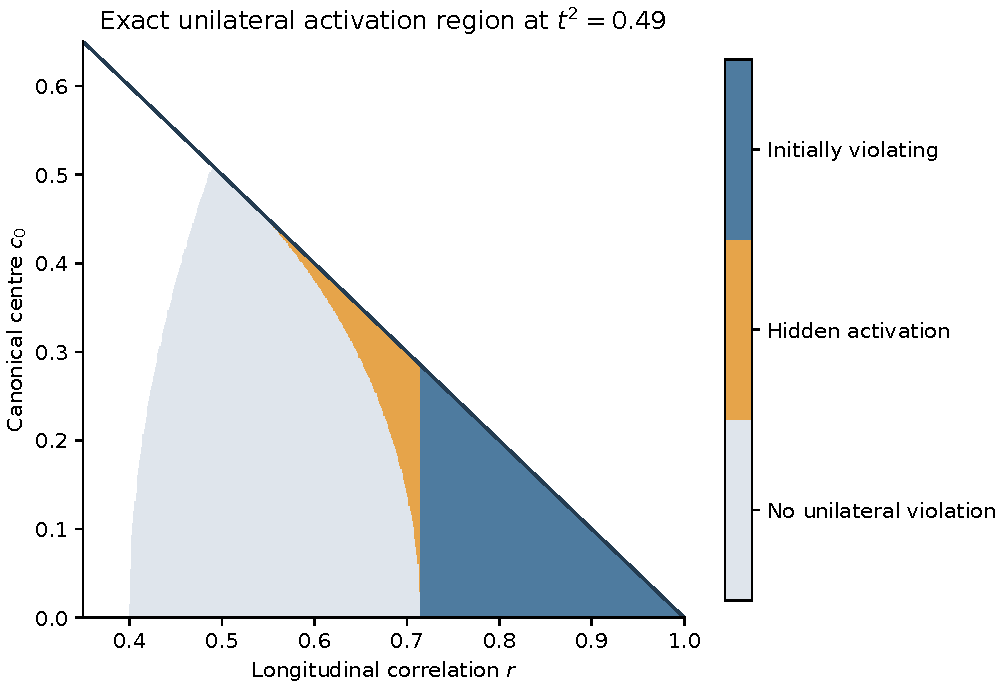
\includegraphics[width=.75\linewidth]{figures/axial_activation_region.pdf}
 \caption{The exact axial activation region at $x=t^2=0.49$.
 The physical region is separated into states with no unilateral
 violation, states with hidden activation, and states that already
 violate CHSH. The boundaries are given by
 \eqref{eq:ext-axial-physical} and~\eqref{eq:ext-axial-activation}.}
 \label{fig:ext-axial-region}
\end{figure}

\begin{corollary}[The quasi-distillable family in the target paper]
\label{cor:ext-quasidistillable}
For
\[
 \rho_p=p|\Psi^-\rangle\langle\Psi^-|
              +(1-p)|00\rangle\langle00|,\qquad 0\le p\le1,
\]
one has
\begin{equation}
 \boxed{\quad
 (B_A^*(\rho_p))^2=(B_B^*(\rho_p))^2
 =\max\left\{1,\frac{2p}{2-p}\right\}.
 \quad}
 \label{eq:ext-quasidistillable}
\end{equation}
For $0<p<2/3$, the value one is a supremum attained only by a
rank-one limit. At and above $p=2/3$, an invertible whitening filter
attains the optimum. At $p=0$, the state is already a pure product.
\end{corollary}

\begin{proof}
For $p>0$, Alice whitening and a local rotation produce the amplitude
damping form $x=r$, $c_0=1-r$, with $r=p/(2-p)$.
The density matrix has rank two, so its boundary value is one.
For $r<1/2$, $\alpha=4r-1<1$, and
Theorem~\ref{thm:ext-threshold} gives exactly one with no finite
attainment. At $r=1/2$, the canonical state already has $B^2=2r=1$.
For $r>1/2$, formula~\eqref{eq:ext-axial-value} has maximum $2r$:
the inequality for the other branch reduces to
$(2r-1)(r-1)\le0$. Symmetry of $\rho_p$ exchanges Alice and Bob.
\end{proof}

This gives a conjecture-free, sharp interval of locally inaccessible hidden
CHSH violation for this family: $0<p\le2/3$.
For comparison, both steering-ellipsoid centres of $\rho_p$ have length
$2(1-p)/(2-p)$, which is at least $1/2$ exactly when $p\le2/3$. Result~1
of~\cite{ducuara} derives the absence of one-sided violation for centre
lengths above $1/2$ from Conjecture~1 of~\cite{milne}, and at centre
length $1/2$ that conjecture also gives $B\le1$; the Omega Institute's
public record of a claimed proof of Conjecture~1~\cite{dossier}
therefore already makes the inaccessibility of $0<p\le2/3$
unconditional, and no priority is claimed for it. What the corollary adds
is the exact value~\eqref{eq:ext-quasidistillable} and the sharpness of the
endpoint: for every $p>2/3$ whitening alone gives a one-sided violation. Indeed, the physical bilateral
filters $F_\varepsilon=\diag(\varepsilon,1)$ on both parties, with
$0<\varepsilon\le1$, produce the same family with parameter and success
probability
\[
 q=\frac{p}{p+(1-p)\varepsilon^2},\qquad
 p_{\rm succ}=p\varepsilon^2+(1-p)\varepsilon^4.
\]
For every $p>0$, $q\to1$ as $\varepsilon\to0$, so the bilateral CHSH supremum
is $\sqrt2$. Directly,
$B(\rho_q)^2=\max\{2q^2,q^2+(1-2q)^2\}$.
For $0<p<1$, the explicit sufficient and necessary condition
$q>1/\sqrt2$ is obtained by choosing
$\varepsilon^2<p(\sqrt2-1)/(1-p)$. Thus every $0<p\le2/3$ permits a
finite-success bilateral violation although neither unilateral filter can
violate. For the exact example $p=3/5$ and $\varepsilon=1/2$, the initial
squared CHSH value is $18/25$, both unilateral suprema have square one,
and the bilateral filtered value has square $72/49$, at success probability
$7/40$. A separate exact rational certificate is included.

The amplitude-damping threshold $r>1/2$ and the loss-channel
golden-ratio threshold are established special cases in
Appendix B of~\cite{zhang}; they are not being claimed as new here.
For example, setting $x=r^2$ and $c_0=1-r$ in
\eqref{eq:ext-axial-activation} gives
$r>(\sqrt5-1)/2$. The theorem supplies one criterion for the full
three-parameter physical family and its exact hidden-activation region.
